
\documentclass[notes,blackandwhite,mathsans,usenames,dvipsnames]{beamer}

\usepackage{amsmath}
\usepackage{amssymb}
\usepackage{graphicx}
\usepackage{fancybox}
\usepackage{booktabs}
\usepackage{multirow,pxfonts}
\usepackage{cmbright}
\usepackage{xcolor}
\usepackage{color}
\usepackage{enumitem}
\usepackage{animate}
\usepackage{changepage}

\usepackage[T1]{fontenc}
\fontencoding{T1}  
\usepackage[utf8]{inputenc}


\usefonttheme{default}
\setbeamercovered{invisible}
\beamertemplatenavigationsymbolsempty

\makeatletter
\setbeamertemplate{footline}
{
  \leavevmode
  \hbox{
  \begin{beamercolorbox}[wd=0.97\paperwidth,ht=2.25ex,dp=2ex,right]{}
{\color{mcxs2} \insertframenumber{} / \inserttotalframenumber}
  \end{beamercolorbox}}%
}


\definecolor{mcxs1}{HTML}{05386B}
\definecolor{mcxs2}{HTML}{379683}
\definecolor{mcxs3}{HTML}{5CDB95}
\definecolor{mcxs4}{HTML}{8EE4AF}
\definecolor{mcxs5}{HTML}{EDF5E1}
\setbeamercolor{frametitle}{fg=mcxs2}
\AtBeginDocument{\color{mcxs1}}
\setbeamertemplate{itemize item}[triangle]


\begin{document}
%\fontfamily{pag}\selectfont
%\setbeamerfont{title}{family=\fontfamily{pag}\selectfont}
%\setbeamerfont{frametitle}{family=\fontfamily{pag}\selectfont}
%\setbeamerfont{framesubtitle}{family=\fontfamily{pag}\selectfont}







{\setbeamercolor{background canvas}{bg=mcxs5}
\begin{frame}

\vspace{1cm}
\begin{tabular}{rl}
&\textbf{\LARGE\color{mcxs3} Macroeconometrics}\\[8ex]
\textbf{\Large Lecture 18}&\textbf{\Large\color{mcxs2}Unobserved Component Model}\\[1ex] &\textbf{\Large\color{mcxs2}Extensions}\\[15ex]
&\textbf{Tomasz Wo\'zniak}\\[1ex]
&{\small\color{mcxs2} Department of Economics}\\
&{\small\color{mcxs2}University of Melbourne}
\end{tabular}

\end{frame}
}




{\setbeamercolor{background canvas}{bg=mcxs5}
\begin{frame}

\vspace{1cm}\textbf{\color{mcxs2}Simulation smoother for band matrix}

\bigskip\textbf{\color{mcxs1}Hierarchical priors for variances}

\bigskip\textbf{\color{mcxs2}Autoregressive slopes from a stationary region}

\bigskip\textbf{\color{mcxs2}Correlated trend and cycle}

\bigskip\textbf{\color{mcxs2}Deterministic or stochastic trend}

\bigskip\textbf{\color{mcxs2}Time-varying drift}


%\vspace{1cm} Useful readings: \footnotesize
%
%\smallskip{\color{mcxs2}Stock \& Watson (2016) Core Inflation and Trend Inflation, Review of Economics and Statistics}

%\normalsize
%\vspace{1cm} Materials: \scriptsize
%
%\smallskip{\color{mcxs2}A zip file} \texttt{L18 mcxs.zip} {\color{mcxs2}for the reproduction of the results}

\end{frame}
}



{\setbeamercolor{background canvas}{bg=mcxs5}
\begin{frame}

\bigskip\textbf{\color{mcxs1}Objectives.}
\begin{itemize}[label=$\blacktriangleright$]
\item {\color{mcxs1}To achieve flexibility in the model specification}
\item {\color{mcxs1}To extend the model by crucial features}
\item {\color{mcxs1}To estimate the extended models}
\end{itemize}

\bigskip\textbf{\color{mcxs2}Learning outcomes.}
\begin{itemize}[label=$\blacktriangleright$]
\item {\color{mcxs2}Modeling flexibility reflecting data properties}
\item {\color{mcxs2}Constructing new estimation algorithms}
\item {\color{mcxs2}Understanding how great UC models can be}
\end{itemize}

\end{frame}
}








\begin{frame}{A simple UC-AR model}

\smallskip\textbf{UC-AR(p) model.}
\begin{align*}
y_t &= \tau_t + \epsilon_t\\[1ex]
\tau_t &= \mu + \tau_{t-1} + \eta_t\\[1ex]
\epsilon_t &= \alpha_1\epsilon_{t-1} + \dots + \alpha_p\epsilon_{t-p} +  e_t\\[2ex]
\begin{bmatrix}\eta_t \\ e_t\end{bmatrix}&\bigg|Y_{t-1} \sim ii\mathcal{N}\left(\mathbf{0}_2, \begin{bmatrix}\sigma_\eta^2 & 0 \\ 0 & \sigma_e^2\end{bmatrix} \right)
\end{align*}

\end{frame}




\begin{frame}{A simple UC-AR model}

\bigskip\textbf{Prior distributions.}\small
\begin{align*}
p(\tau,\epsilon,\alpha,\beta,\sigma) &= p\left(\tau|\beta,\sigma^2_\eta\right)p(\beta)p\left(\sigma^2_\eta\right)
p\left(\epsilon|\alpha,\sigma^2_e\right)p(\alpha)p\left(\sigma^2_e\right)\\[2ex]
\tau|\beta,\sigma^2_\eta &\sim\mathcal{N}\left(H^{-1} X_\tau \beta, \sigma^2_\eta (H'H)^{-1}\right)\\
\beta&\sim\mathcal{N}_2\left(\underline{\beta},\underline{V}_{\beta}\right)\\
\sigma^2_\eta&\sim\mathcal{IG}2\left(\underline{s},\underline{\nu}\right)\\[2ex]
\epsilon|\alpha,\sigma^2_e &\sim\mathcal{N}\left(\mathbf{0}_T, \sigma^2_e (H_{\alpha}'H_{\alpha})^{-1}\right)\\
\alpha&\sim\mathcal{N}_p\left(\underline{\alpha},\underline{V}_{\alpha}\right)\mathcal{I}(\alpha\in A)\\
\sigma^2_e&\sim\mathcal{IG}2\left(\underline{s},\underline{\nu}\right)
\end{align*}

\end{frame}







{\setbeamercolor{background canvas}{bg=mcxs5}
\begin{frame}

\begin{adjustwidth}{-0.5cm}{0cm}
\vspace{8.3cm}
\Large\textbf{{\color{mcxs2}Simulation smoother} {\color{mcxs3} for band matrix}}
\end{adjustwidth}

\end{frame}
}


\begin{frame}[fragile]{Simulation smoother for band matrix}

{\color{mcxs2}When the autoregressive lag order is greater than} $p\geq2$ {\color{mcxs2}the precision matrix of the full conditional posterior distributions for} $\tau$ {\color{mcxs2}and} $\epsilon$ {\color{mcxs2}is not tridiagonal but} band.

\smallskip{\color{mcxs2}Use functions} \texttt{bandchol}, \texttt{forwardsolve} {\color{mcxs2}and} \texttt{backsolve} {\color{mcxs2}from package} \texttt{mgcv}

\begin{verbatim}
library(mgcv)

N           = dim(D)[1]
D.L         = t(bandchol(D))
x           = rnorm(N)

a           = forwardsolve(D.L, b)
draw        = backsolve(t(D.L), a + x)
\end{verbatim}

\end{frame}





{\setbeamercolor{background canvas}{bg=mcxs5}
\begin{frame}

\begin{adjustwidth}{-0.5cm}{0cm}
\vspace{8.3cm}
\Large\textbf{{\color{mcxs2}Hierarchical priors} {\color{mcxs3} for variances}}
\end{adjustwidth}

\end{frame}
}




\begin{frame}{Hierarchical priors for variances}

\textbf{Priors might drive the posterior results.}

\smallskip{\color{mcxs2}Extensive latent structure of UC models might make the dependence of the posterior results on prior assumptions strong. 

\bigskip Choosing arbitrary values of the prior distribution parameters might drive the definition, estimates, and the interpretation of the trend and cyclical components.
}

\bigskip\textbf{A solution.} 

\smallskip{\color{mcxs2}Extend the hierarchy of the prior distributions, specify a prior distribution for} $\underline{s}${\color{mcxs2}, and estimate it. }

\bigskip{\color{mcxs2}The hierarchical prior for the model's variances is given by}
\begin{align*}
p\left( \sigma^2_\eta \mid {\color{purple}\underline{s}} \right) p\left( \sigma^2_e \mid {\color{purple}\underline{s}} \right) {\color{purple}p\left( \underline{s} \right)}
\end{align*}
\end{frame}





\begin{frame}{Hierarchical priors for variances}

\bigskip\textbf{The prior.}

\smallskip{\color{mcxs2}The conditionally-conjugate prior for} ${\color{purple}\underline{s}}$ {\color{mcxs2}is the gamma distribution.}
\begin{align*}
{\color{purple}\underline{s}}&\sim \mathcal{G}(s,a) \quad\propto\quad  {\color{purple}\underline{s}}^{a-1}\exp\left\{ -\frac{{\color{purple}\underline{s}}}{s} \right\}\\
E[{\color{purple}\underline{s}}]&=as\\
Var[{\color{purple}\underline{s}}]&=as^2 
\end{align*}


\bigskip\textbf{The hierarchy.}
\begin{align*}
\sigma^2_\eta|{\color{purple}\underline{s}} &\sim\mathcal{IG}2({\color{purple}\underline{s}},\underline{\nu})
\qquad\propto {\color{purple}\underline{s}}^{\frac{\underline\nu}{2}}\left(\sigma^2_\eta\right)^{-\frac{\underline\nu+2}{2}}\exp\left\{-\frac{1}{2}\frac{{\color{purple}\underline{s}}}{\sigma^2_\eta} \right\}
\\
\sigma^2_e|{\color{purple}\underline{s}} &\sim\mathcal{IG}2({\color{purple}\underline{s}},\underline{\nu})
\qquad\propto {\color{purple}\underline{s}}^{\frac{\underline\nu}{2}}\left(\sigma^2_e\right)^{-\frac{\underline\nu+2}{2}}\exp\left\{-\frac{1}{2}\frac{{\color{purple}\underline{s}}}{\sigma^2_e} \right\}
\\
{\color{purple}\underline{s}}&\sim\mathcal{G}(s,a)\quad\quad\quad
\propto {\color{purple}\underline{s}}^{a-1}\exp\left\{ -\frac{{\color{purple}\underline{s}}}{s}\right\}
\end{align*}

\end{frame}





\begin{frame}{Hierarchical priors for variances}

\bigskip\textbf{Full conditional posterior distribution.}

\smallskip{\color{mcxs2}The Gibbs sampler has to be extended by one more step:}
\begin{align*}
{\color{purple}\underline{s}}|y,\sigma^2_\eta, \sigma^2_e &\sim\mathcal{G}\left( \left(s^{-1} + 0.5\left(\sigma^{-2}_\eta + \sigma^{-2}_e\right)\right)^{-1}, \underline\nu+a	\right)
\end{align*}

\end{frame}








{\setbeamercolor{background canvas}{bg=mcxs5}
\begin{frame}

\begin{adjustwidth}{-0.5cm}{0cm}
\vspace{8.3cm}
\Large\textbf{{\color{mcxs2}Autoregressive slopes} {\color{mcxs1}from a stationary region}}
\end{adjustwidth}

\end{frame}
}



\begin{frame}{Autoregressive slopes from a stationary region}

\bigskip{\color{mcxs2}Sampling autoregressive slope parameters} $\alpha$ {\color{mcxs2}from the stationary region} $\alpha\in A$ {\color{mcxs2}might be non-trivial}

\bigskip {\color{mcxs2}Begin with a simple case of} $p=1$ {\color{mcxs2}with} $\alpha_1\in(-1,1)$

\bigskip {\color{mcxs2}Assume a truncated normal prior}
$$
\alpha_1 \sim\mathcal{N}\left( \underline{\alpha}_1 ,\underline{V}_{\alpha}\right)\mathcal{I}(\alpha_1\in (-1,1))
$$

\bigskip {\color{mcxs2}Sample it from a univariate truncated normal distribution}
\begin{align*}
p\left( \alpha|y,\epsilon,\sigma^2_e \right) &= \mathcal{N}_p\left(\overline{\alpha},\overline{V}_\alpha\right)\mathcal{I}(\alpha\in (-1,1))\\
\overline{V}_\alpha &= \left[\sigma^{-2} _e X_\epsilon' X_\epsilon + \underline{V}_\alpha^{-1} \right]^{-1}\\
\overline{\alpha} &= \overline{V}_\alpha \left[\sigma^{-2} _e X_\epsilon' \epsilon + \underline{V}_\alpha^{-1}\underline{\alpha}  \right]
\end{align*}
{\color{mcxs2}Using function} \texttt{RcppTN::rtn}

\end{frame}





\begin{frame}{Autoregressive slopes from a stationary region}

{\color{mcxs2}A recommended strategy for the case of} $p\geq2$ {\color{mcxs2}is to not impose the restrictions in the sampler.}


\bigskip{\color{mcxs2}The benefits are}
\begin{description}
\item[No tedious sampler] {\color{mcxs2}taking forever to run when the true probability of} $\alpha\in A$ {\color{mcxs2}is not equal to} 1

\smallskip\item[If is not such that $\alpha\in A$] {\color{mcxs2}then} $y_t$ {\color{mcxs2}has more than one unit root and the trend and cycle are not identified in a simple UC model. Need to refine the model anyways.}
\end{description}

\end{frame}













{\setbeamercolor{background canvas}{bg=mcxs5}
\begin{frame}

\begin{adjustwidth}{-0.5cm}{0cm}
\vspace{8.3cm}
\Large\textbf{{\color{mcxs2}Correlated } {\color{mcxs1}trend and cycle}}
\end{adjustwidth}

\end{frame}
}



\begin{frame}{Correlated trend and cycle}


{\color{mcxs2}When the autoregressive lag order is greater than} $p\geq2$ {\color{mcxs2}the covariance between shocks} $\eta_t$ {\color{mcxs2}and} $e_t$ {\color{mcxs2}is identified and can be estimated.

\bigskip Appropriate parameterisation of a model makes the estimation fast and simple.
}

\bigskip\textbf{Error term specification.}
\begin{align*}
\begin{bmatrix}\eta_t \\ e_t\end{bmatrix}&\bigg|Y_{t-1} \sim ii\mathcal{N}\left(\mathbf{0}_2, \Sigma \right)\\[2ex]
\Sigma &= \begin{bmatrix}\sigma_\eta^2 & {\color{purple}\rho \sigma_\eta \sigma_e} \\  & \sigma_e^2\end{bmatrix}\\[2ex]
{\color{purple}\rho}&\text{ -- correlation between the shocks} 
\end{align*}

\end{frame}





\begin{frame}{Correlated trend and cycle}

{\color{mcxs2}The implementation is based on the decomposition of the joint bivariate normal distribution into  conditional and marginal distributions.}
\begin{align*}
\begin{bmatrix}x_1\\ x_2\end{bmatrix}&\sim\mathcal{N}\left(\begin{bmatrix}\mu_1\\ \mu_2\end{bmatrix},\begin{bmatrix}\sigma_1^2& \rho\sigma_1\sigma_2\\&\sigma_2^2\end{bmatrix}\right)\\[1ex]
&\downarrow\\[1ex]
x_1\mid x_2 &\sim \mathcal{N}\left( \mu_1 + \rho\frac{\sigma_1}{\sigma_2}x_2, \left(1-\rho^2\right)\sigma_1^2\right)\\
x_2 &\sim \mathcal{N}\left( \mu_2, \sigma_2^2\right)
\end{align*}

\end{frame}





\begin{frame}{Correlated trend and cycle}

\bigskip {\color{mcxs2}The model in its original form} \small
\begin{align*}
y &= \tau + \epsilon \tag{1}\\[1ex]
H\tau &=  X_\tau \beta + \eta\tag{2}\\
H_\alpha \epsilon &=  e\tag{3}\\[1ex]
\begin{bmatrix}\eta \\ e\end{bmatrix}\bigg|y &\sim \mathcal{N}_{2T}\left(\mathbf{0}_{2T}, \begin{bmatrix}\sigma_\eta^2 & {\color{purple}\rho \sigma_\eta \sigma_e} \\  & \sigma_e^2\end{bmatrix} \otimes I_T\right) \tag{4 \& 5}
\end{align*}

\normalsize\bigskip {\color{mcxs2}is rewritten as} \small
\begin{align*}
H\tau &=  X_\tau \beta  +  {\color{purple}\rho \frac{\sigma_\eta}{ \sigma_e} e} + \eta\tag{2}\\
H_\alpha \epsilon &=  e\tag{3}\\[1ex]
\eta \mid e &\sim \mathcal{N}_{T}\left(\mathbf{0}_{T}, \left(1-\rho^2\right)\sigma_\eta^2  I_T\right)\tag{4}\\
e &\sim \mathcal{N}_{T}\left(\mathbf{0}_{T}, \sigma_e^2  I_T\right)\tag{5}
\end{align*}

\end{frame}






\begin{frame}{Correlated trend and cycle}

\normalsize\bigskip {\color{mcxs2}The modifications include defining new matrices and parameters} \small
\begin{align*}
\tilde{X}_\tau &= \begin{bmatrix}\imath_t&e_{1.T}&{\color{purple}e}\end{bmatrix} &\tilde\beta &= \begin{bmatrix}\mu & \tau_0 &{\color{purple}\gamma}\end{bmatrix}'\\[1ex]
{\color{purple}\gamma} &= \rho\frac{\sigma_\eta}{\sigma_e} &{\color{purple}\tilde\sigma_\eta^2} &= \left(1-\rho^2\right)\sigma_\eta^2 
\end{align*}\normalsize
{\color{mcxs2}... and rewriting the model}\small
\begin{align*}
H\tau &=  \tilde{X}_\tau \tilde\beta + \eta &&\tag{2}\\
\eta \mid e &\sim \mathcal{N}_{T}\left(\mathbf{0}_{T}, {\color{purple}\tilde\sigma_\eta^2}  I_T\right)&&\tag{4}
\end{align*}

\normalsize \bigskip{\color{mcxs2}The interpretable parameters of the model can be retrieved by} \small
$$ \sigma_\eta^2 = \tilde\sigma_\eta^2 + \gamma^2\sigma_e^2 \qquad
\rho = \gamma\frac{\sigma_e}{\sqrt{\tilde\sigma_\eta^2 + \gamma^2\sigma_e^2}}$$

\normalsize {\color{mcxs2}The Gibbs sampler stays the same after replacing} $\tilde{X}_\tau$ {\color{mcxs2}for} $X_\tau$, $\tilde\beta$ {\color{mcxs2}for} $\beta${\color{mcxs2}, and} $\tilde\sigma_\eta^2$ {\color{mcxs2}for} $\sigma_\eta^2$.
\end{frame}










{\setbeamercolor{background canvas}{bg=mcxs5}
\begin{frame}

\begin{adjustwidth}{-0.5cm}{0cm}
\vspace{8.3cm}
\Large\textbf{{\color{mcxs2}Deterministic or} {\color{mcxs3} stochastic trend}}
\end{adjustwidth}

\end{frame}
}





\begin{frame}{Deterministic or stochastic trend}


\bigskip\textbf{Autoregressive model} obtained by imposing $\sigma_\eta^2=0$
$$
\begin{array}{rl}
y_t -\mu t &= \epsilon_t\\[1ex]
\alpha_p(L)\epsilon_t &=  e_t\\[1ex]
e_t |Y_{t-1} &\sim iid\mathcal{N}\left(0,\sigma_e^2\right)
\end{array}
$$

\textbf{Alternative hypotheses.}

\begin{description}
\item[$\sigma_\eta^2\neq 0$] {\color{mcxs2}-- trend-cycle decomposition of unit-root non-stationary series with on unit root}

\smallskip\item[$\sigma_\eta^2=0$] {\color{mcxs2}-- unit-root stationary cycle around a deterministic trend}
\end{description}


\end{frame}






\begin{frame}{Deterministic or stochastic trend}


\textbf{Gamma prior for $\sigma^2_\eta$.}

\smallskip{\color{mcxs2}The possibility of of shrinking the value of variance to} zero {\color{mcxs2}is facilitated by a gamma prior the shape parameter set to} $\frac{1}{2}$ 

$$\sigma_\eta^2\mid \underline{s}\sim\mathcal{G}\left(2\underline{s}, \frac{1}{2}\right)$$ 

\bigskip{\color{mcxs2}where} $E[\sigma_\eta^2] = \underline{s}$ {\color{mcxs2}and} $\underline{s}$ {\color{mcxs2}is a hyper-parameter to be specified}

\bigskip{\color{mcxs2}}

\end{frame}



\begin{frame}{Deterministic or stochastic trend}

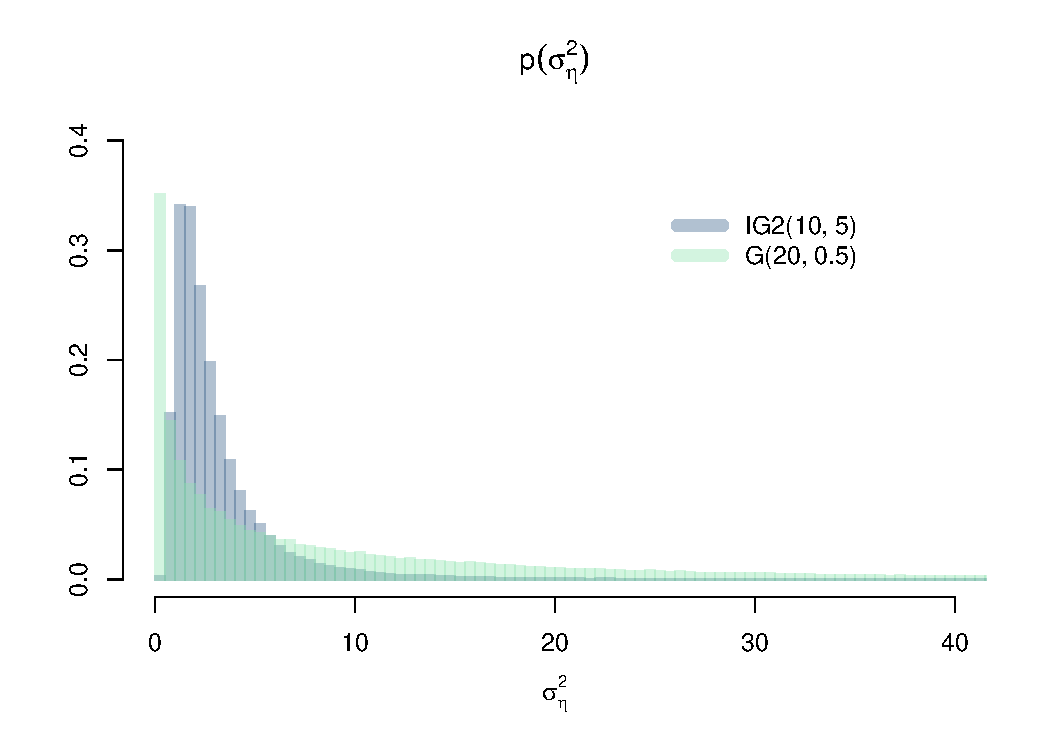
\includegraphics[scale=0.65, trim = 1cm 1cm 1cm 0cm]{prior_sigma2eta}

\end{frame}



\begin{frame}{Deterministic or stochastic trend}

\bigskip
\begin{center}
\textbf{Implied prior for $\tau_t$ assuming $\mu=0$}

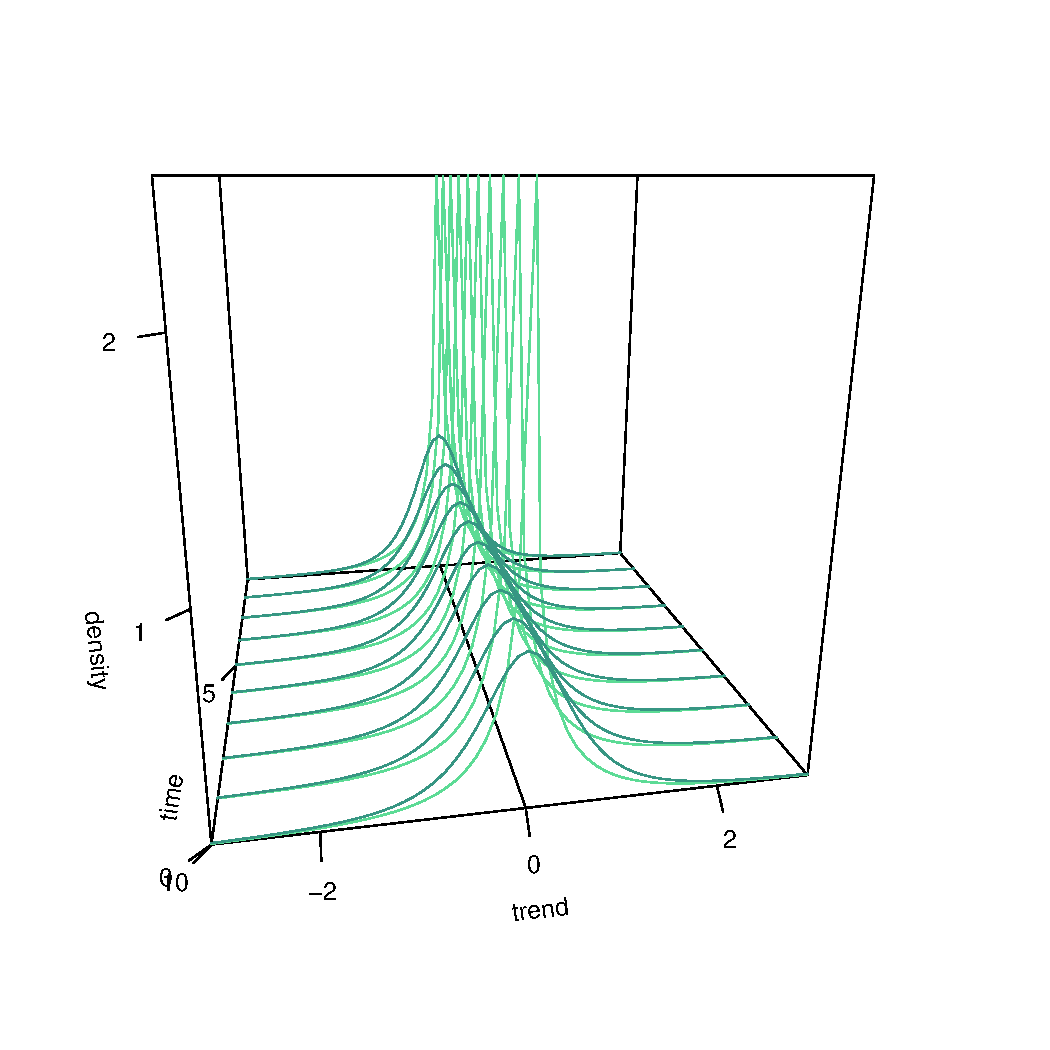
\includegraphics[scale=0.55, trim = 1cm 1cm 1cm 2cm]{prior_trend.pdf}
\end{center}
\end{frame}




\begin{frame}{Deterministic or stochastic trend}

\textbf{Full conditional posterior density.}

\smallskip{\color{mcxs2}The gamma prior implies a generalised inverse Gaussian full conditional posterior distribution for} $\sigma_\eta^2$

\begin{align*}
p\left(\sigma_\eta^2 \mid y, \tau, \beta \right) &= \mathcal{GIG}\left(\lambda, \chi, \psi \right)\\[1ex]
\lambda &= - \frac{T-1}{2} \\
\chi &= (X_\tau \beta - H\tau)'(X_\tau \beta - H\tau) \\ 
\psi &= \frac{2}{\underline{s}}\\
\end{align*}

{\color{mcxs2}Sample from this distribution using function} \texttt{GIGrvg::rgig}

\end{frame}








{\setbeamercolor{background canvas}{bg=mcxs5}
\begin{frame}

\begin{adjustwidth}{-0.5cm}{0cm}
\vspace{8.3cm}
\Large\textbf{{\color{mcxs2}Time-varying } {\color{mcxs1}drift}}
\end{adjustwidth}

\end{frame}
}





\begin{frame}{Time-varying drift}

{\color{mcxs2}Make the drift parameter change over time} 
\begin{align*}
\tau_t &= \mu_t + \tau_{t-1} + \eta_t\\
\mu_t &= \mu_{t-1} + m_t\\[1ex]
m_t|Y_{t-1} &\sim \mathcal{N}\left(0,\sigma_m^2\right)\\
\sigma_m^2 \mid \underline{s} &\sim\mathcal{IG}2(\underline{s},\underline{\nu})
\end{align*}
{\color{mcxs2}The time-varying intercept parameter} $\mu_t$ {\color{mcxs2}follows a Gaussian random walk process with initial value} $\mu_0$

\bigskip{\color{mcxs2}Unit-root non-stationarity of} $\mu_t$ {\color{mcxs2}require the series} $y_t$ {\color{mcxs2}to have two unit roots}

\bigskip{\color{mcxs2}This might be a perfect model for} \emph{CPI prices}
\end{frame}





\begin{frame}{Time-varying drift}

\smallskip{\color{mcxs2}Define} $T\times1$ {\color{mcxs2}matrices} $\mu=\begin{bmatrix} \mu_1&\hdots&  \mu_T\end{bmatrix}'$ {\color{mcxs2}and} $m=\begin{bmatrix}m_1& \hdots & m_T\end{bmatrix}'$

\bigskip{\color{mcxs2}Rewrite the trend equation}
\begin{align*}
H\tau &= \mu + e_{1.T}\tau_0 + \eta 
\end{align*}

\smallskip{\color{mcxs2}Specify equations for} $\mu$
\begin{align*}
H\mu &= \mu_0e_{1.T} + m\\
\mu &= \mu_0\imath_{T} + H^{-1}m\\[1ex]
m &\sim \mathcal{N}\left(\mathbf{0}_T, \sigma^2_m I_T\right)
\end{align*}

\end{frame}





\begin{frame}{Time-varying drift}

{\color{mcxs2}Sample} $\tau$ {\color{mcxs2}from a multivariate normal distribution using the simulation smoother}

\begin{align*}
p\left( \tau|y,\alpha,\beta,\sigma \right)&= \mathcal{N}_T\left(\overline{\tau},\overline{V}\right)\\[2ex]
\overline{V} &= \left[\sigma^{-2} _eH'_\alpha H_\alpha + \sigma^{-2} _\eta H' H \right]^{-1}\\
\overline{\tau} &= \overline{V}\left[\sigma^{-2} _eH'_\alpha H_\alpha y + \sigma^{-2} _\eta H' (\mu + \tau_0e_{1.T}) \right]
\end{align*}

\end{frame}






\begin{frame}{Time-varying drift}

{\color{mcxs2}Sample} $\mu$ {\color{mcxs2}from a multivariate normal distribution using the simulation smoother}

\begin{align*}
p\left( \mu|y,\tau,\tau_0,\mu_0,\sigma^2_\eta,\sigma^2_m \right)&= \mathcal{N}_T\left(\overline{\mu},\overline{V}_\mu\right)\\[2ex]
\overline{V}_\mu &= \left[ \sigma_\eta^{-1}I_T + \sigma_m^{-1}H'H \right]^{-1} \\
\overline{\mu} &= \overline{V}_\mu\left[ \sigma_\eta^{-1}(H\tau-e_{1.T}\tau_0) + \sigma_m^{-1}e_{1.T}\mu_0\right]
\end{align*}

\end{frame}






\begin{frame}{Time-varying drift}

\bigskip{\color{mcxs2}Sample} $\mu_0$ {\color{mcxs2}from a normal distribution}
\begin{align*}
p\left( \mu_0|y,\mu,\sigma^2_m \right) &= \mathcal{N}\left(\overline{\mu}_0,\overline{V}_{\mu.0}\right)\\[1ex]
\overline{V}_{\mu.0} &= \left[\sigma^{-2}_m  + \underline{V}_\mu^{-1} \right]^{-1}\\
\overline{\mu}_0 &= \overline{V}_{\mu.0} \left[\frac{\mu_1}{\sigma^{2}_m} + \frac{\underline{\mu}_0}{\underline{V}_\mu}  \right]
\end{align*}

{\color{mcxs2}... and} $\sigma^2_m$ {\color{mcxs2}from the inverse gamma 2}
\begin{align*}
p\left( \sigma^2_m|y,\mu,\mu_0,\underline{s} \right) &= \mathcal{IG}2\left(\overline{s}_m,\overline{\nu}_m\right)\\[1ex]
\overline{s}_m &= \underline{s} + (H\mu-e_{1.T}\mu_0)'(H\mu-e_{1.T}\mu_0)\\
\overline{\nu}_m &= \underline{\nu} + T
\end{align*}

\end{frame}




{\setbeamercolor{background canvas}{bg=mcxs5}
\begin{frame}

\bigskip\textbf{\color{mcxs1}Other extensions and applications of state space models:}
\begin{itemize}[label=$\blacktriangleright$]
\item {\color{mcxs1}handling seasonality in time series}
\item {\color{mcxs1}dynamic factor models capturing the variability of many variables with a few factors}
\item {\color{mcxs1}time-varying parameter models}
\item {\color{mcxs1}Stochastic Volatility}
\end{itemize}

\end{frame}
}



{\setbeamercolor{background canvas}{bg=mcxs5}
\begin{frame}{Unobserved Component Model Extensions}

{\color{mcxs1}UC models are used to introduce to state-space modeling}

\bigskip{\color{mcxs2}Every single extension might make the model suitable for the data 

\bigskip Their various combination result in a flexible setting applicable to a range of economic and financial data}

\end{frame}
}





\end{document} 